\textbf{Análisis de aplicaciones similares}: No es posible mejorar un producto sin analizarlo y criticarlo. Por ende, es necesario comparar el diseño del prototipo del interfaz gráfica de usuario para así mejorarlo en términos de usabilidad y comodidad.

Las aplicaciones que se van a utilizar como objectos de comparación son las mismas que se utilizaron los antecedentes, \textit{FAT - Frame Data!} y \textit{Smash Ultimate Calculator}.

Como se puede apreciar en la figuras \ref{fig: char sel}, \ref{fig: game select}, \ref{fig: compare options} y \ref{fig: comparison}, \textit{FAT - FRAME DATA!} parece utilizar diseño material \cite{noauthor_designing_nodate}. Mas aún, en la figura \ref{fig: char sel}, se utilizan las siluetas de los personajes con el color predominante del personaje como color de fondo. Esto ayuda reducir la carga de memoria de los usuarios mientras que no sacrifica mucho en términos de usabilidad. Es una buena decisión de diseño y es algo que falta en la interfaz gráfica de usuario de SkyboundDB 2.0. Al utilizar principios del diseño material, \textit{FAT - Frame Data!} es inmediatamente familiar a usuarios de aplicaciones de \textit{Google} y \textit{Android}. El uso de diseño material fue una buena decisión de diseño ya que facilita la adaptación de los usuarios a una aplicación nueva porque comparte principios y estándares de diseño.

\begin{figure}
    \centering
    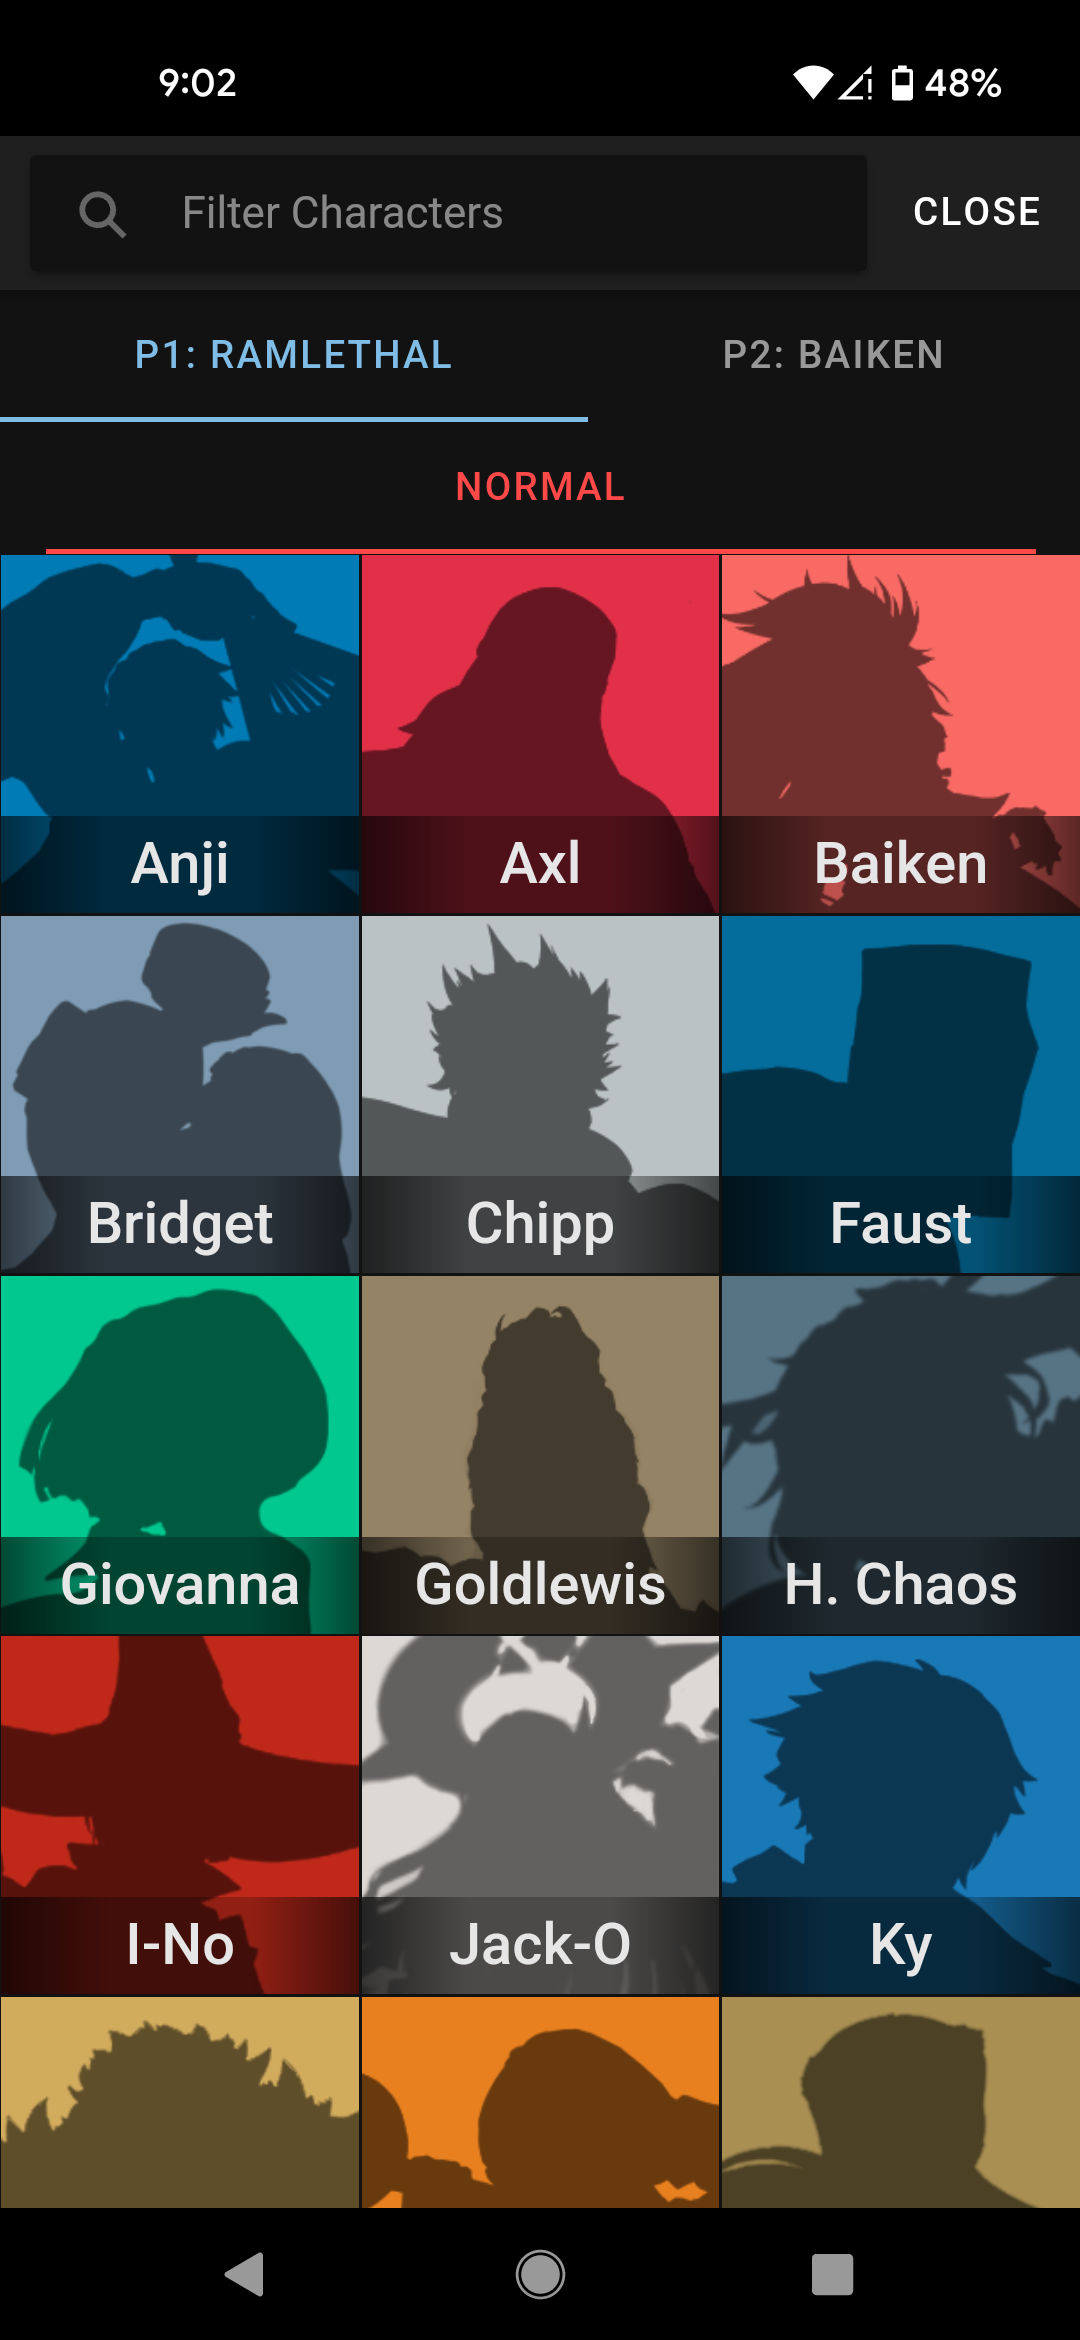
\includegraphics[height=0.4\textheight]{figures/char_sel.png}
    \caption{Selección de personaje en \textit{FAT - FRAME DATA!}}
    \label{fig: char sel}
\end{figure}

\begin{figure}
    \centering
    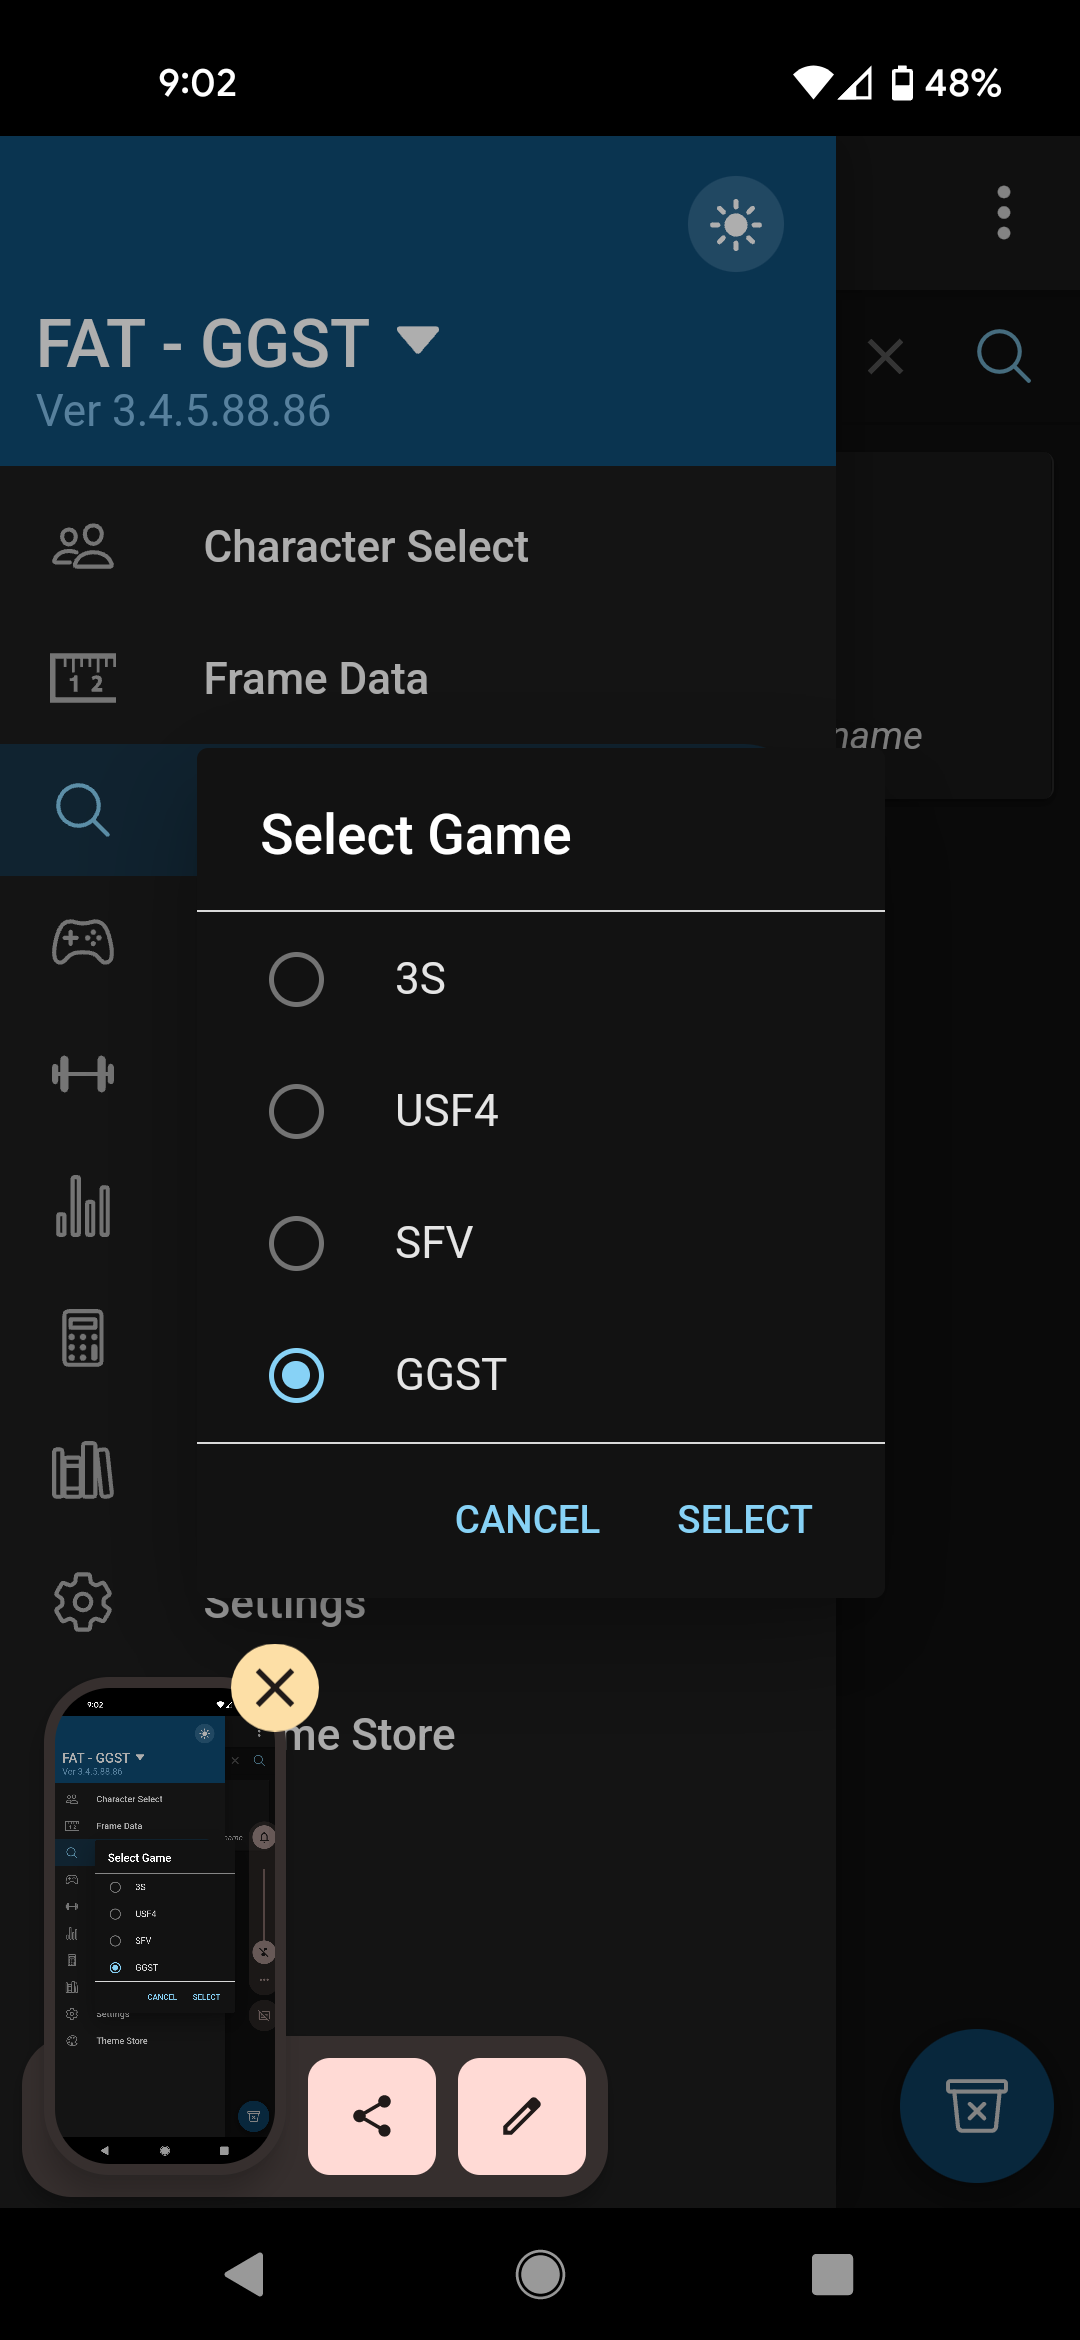
\includegraphics[height=0.4\textheight]{figures/game_options.png}
    \caption{Selección de juego en \textit{FAT - FRAME DATA!}}
    \label{fig: game select}
\end{figure}

\begin{figure}
    \centering
    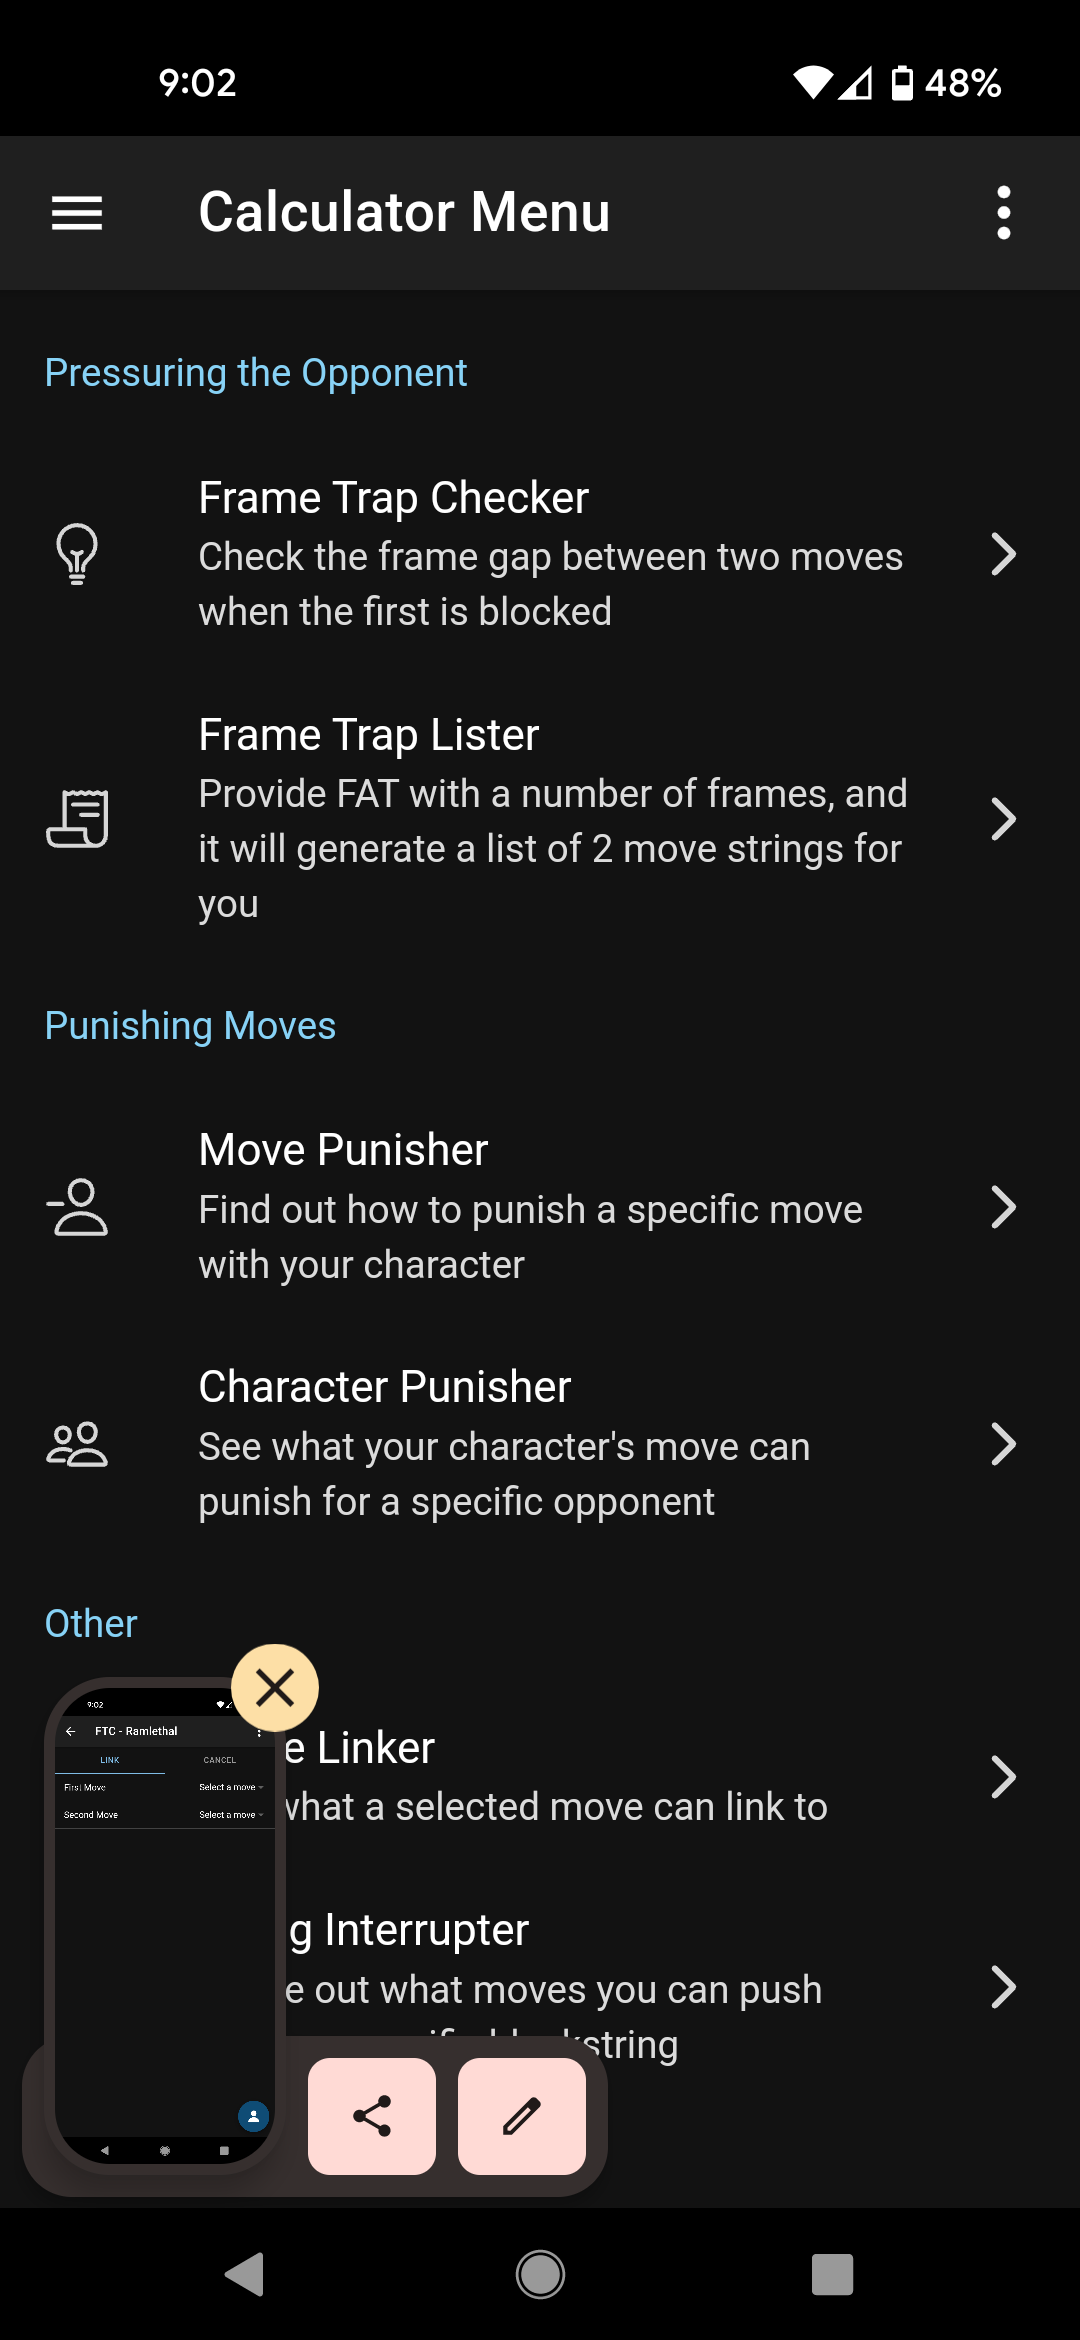
\includegraphics[height=0.4\textheight]{figures/compare_options.png}
    \caption{Opciones de comparación en \textit{FAT - FRAME DATA!}}
    \label{fig: compare options}
\end{figure}

\begin{figure}
    \centering
    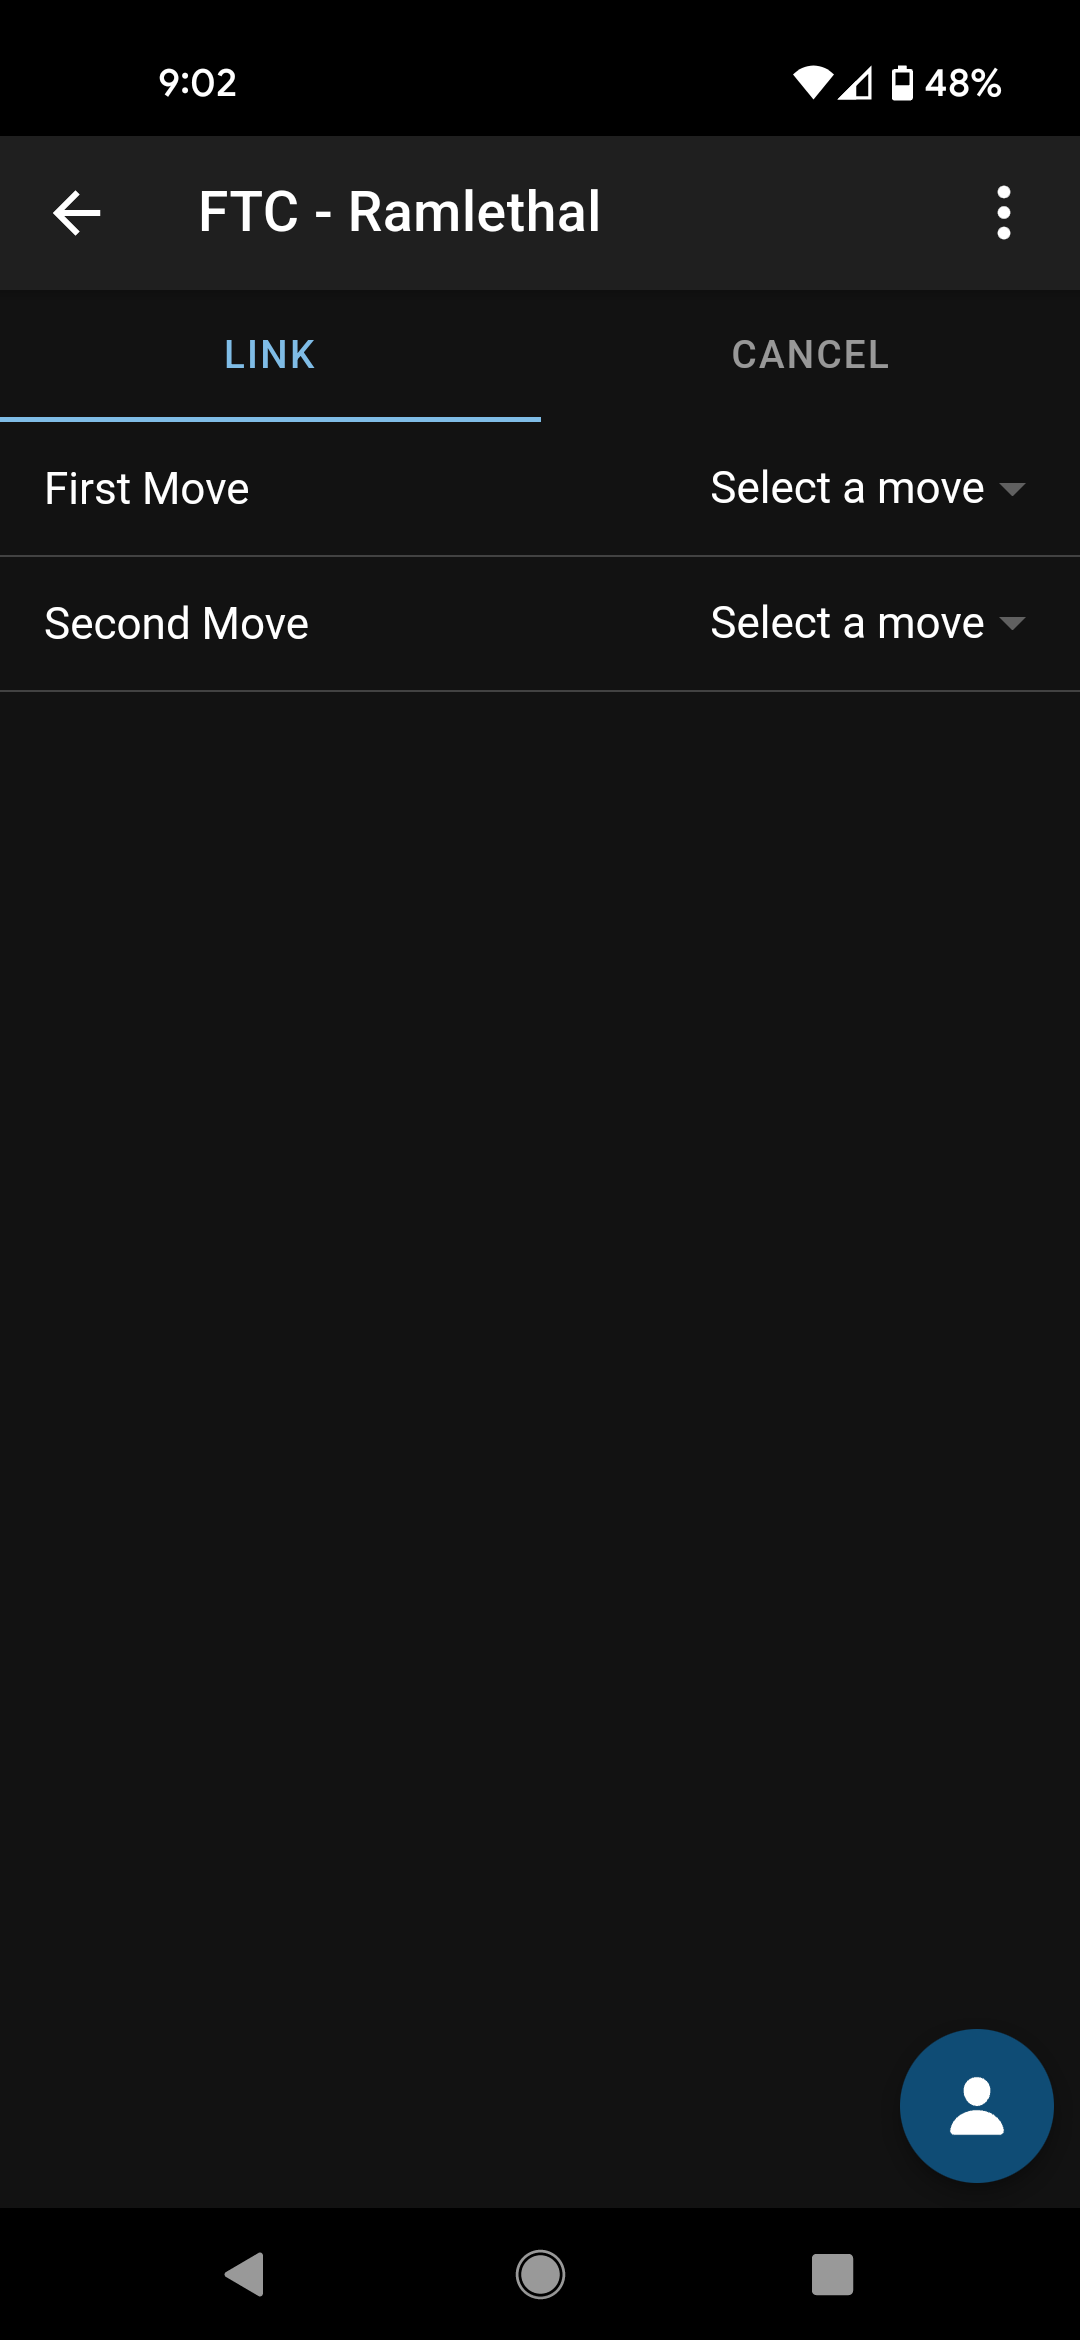
\includegraphics[height=0.4\textheight]{figures/comparison.png}
    \caption{Comparación entre movidas en \textit{FAT - FRAME DATA!}}
    \label{fig: comparison}
\end{figure}

\newpage

\textit{Smash Ultimate Calculator} no parece utilizar un estándar de diseño al igual que SkyboundDB 2.0. Esto crea confusión al utilizar la aplicación por primera vez. Como se puede ver en las figuras \ref{fig: SUC main menu} y \ref{fig: SUC additional options}, a pesar que las areas que contienen información están agrupadas lógicamente, hay demasiados elementos y opciones que se presentan al usuario. Esto incurre una gran carga de memoria e intimida al usuario novato. También es difícil ver que cambios ocurren al oprimir opciones. A pesar de estas decisiones de diseño problemáticas, la paleta de colores es pasable, sino un poco deprimente y sin vida.

\begin{figure}[ht!]
    \centering
    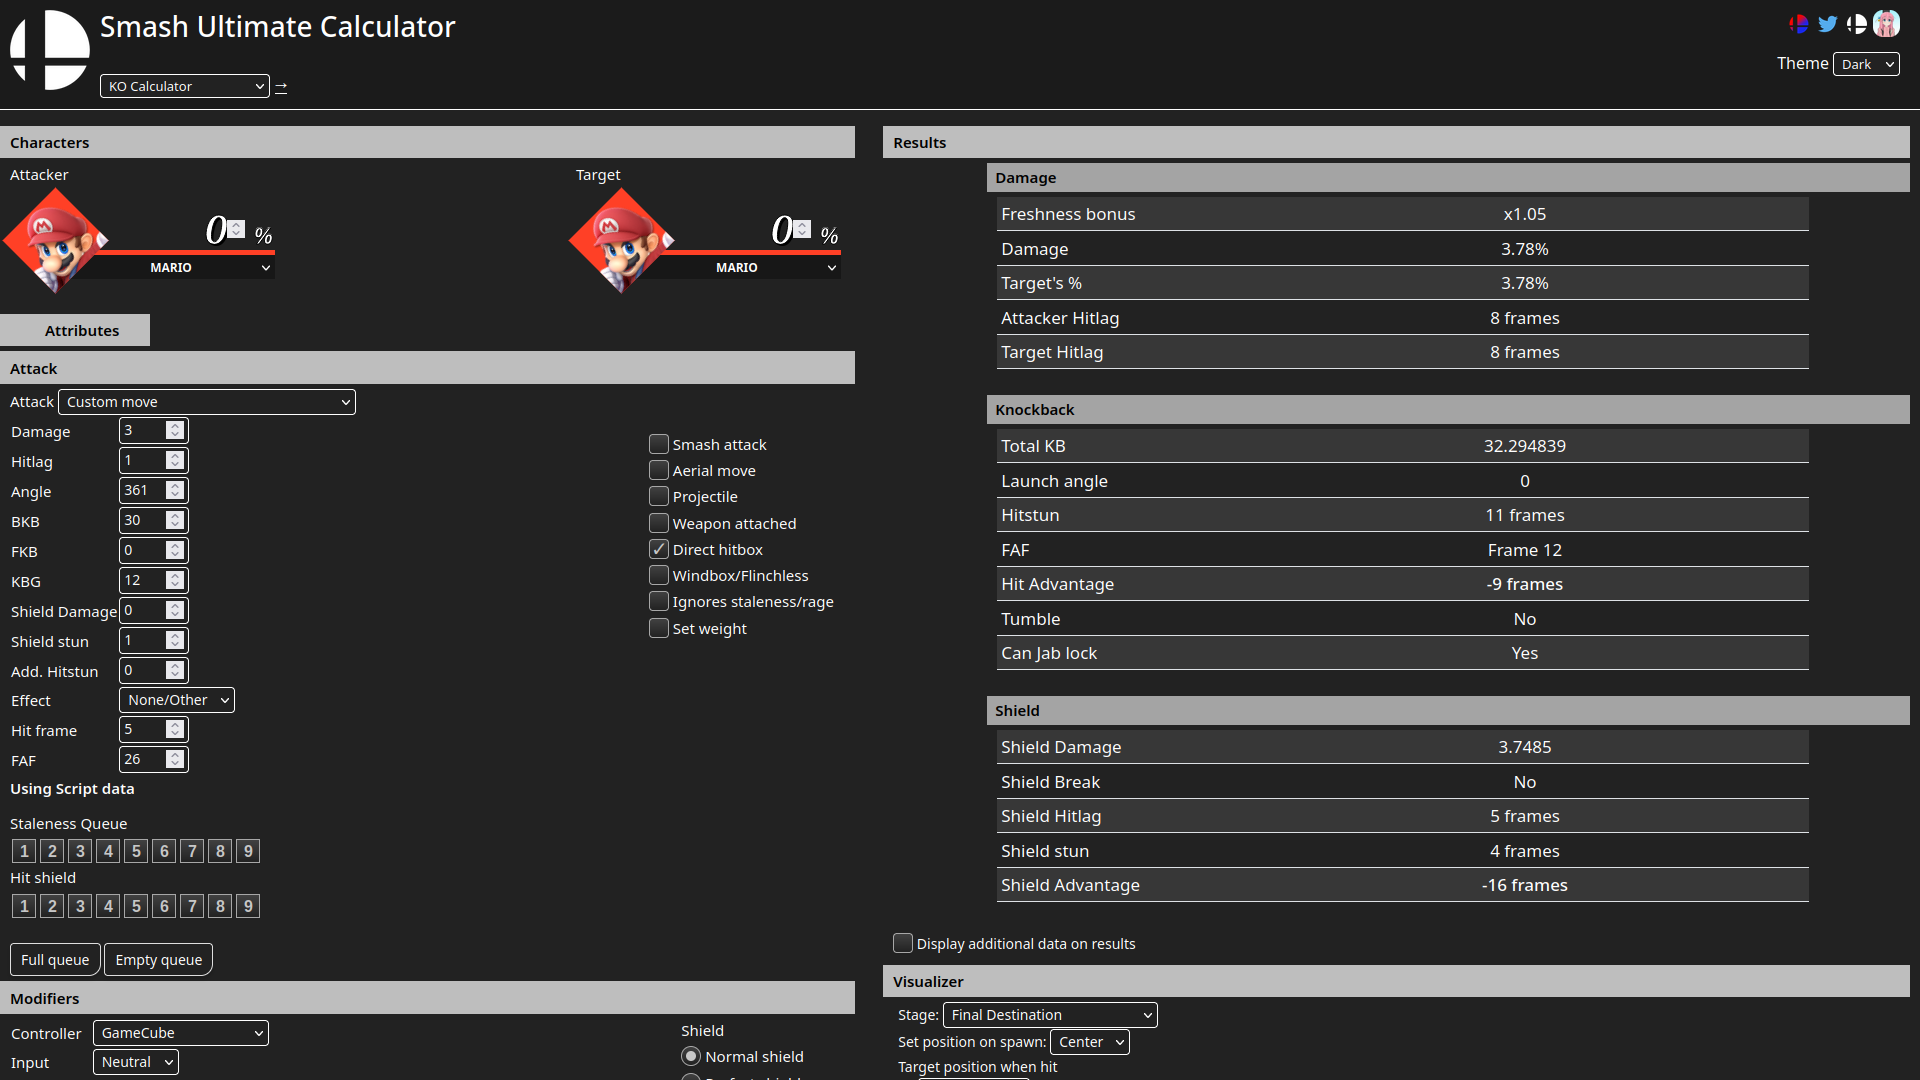
\includegraphics[width=\textwidth]{figures/SUC1.png}
    \caption{Menú principal de \textit{Smash Ultimate Calculator}}
    \label{fig: SUC main menu}
\end{figure}

\begin{figure}[ht!]
    \centering
    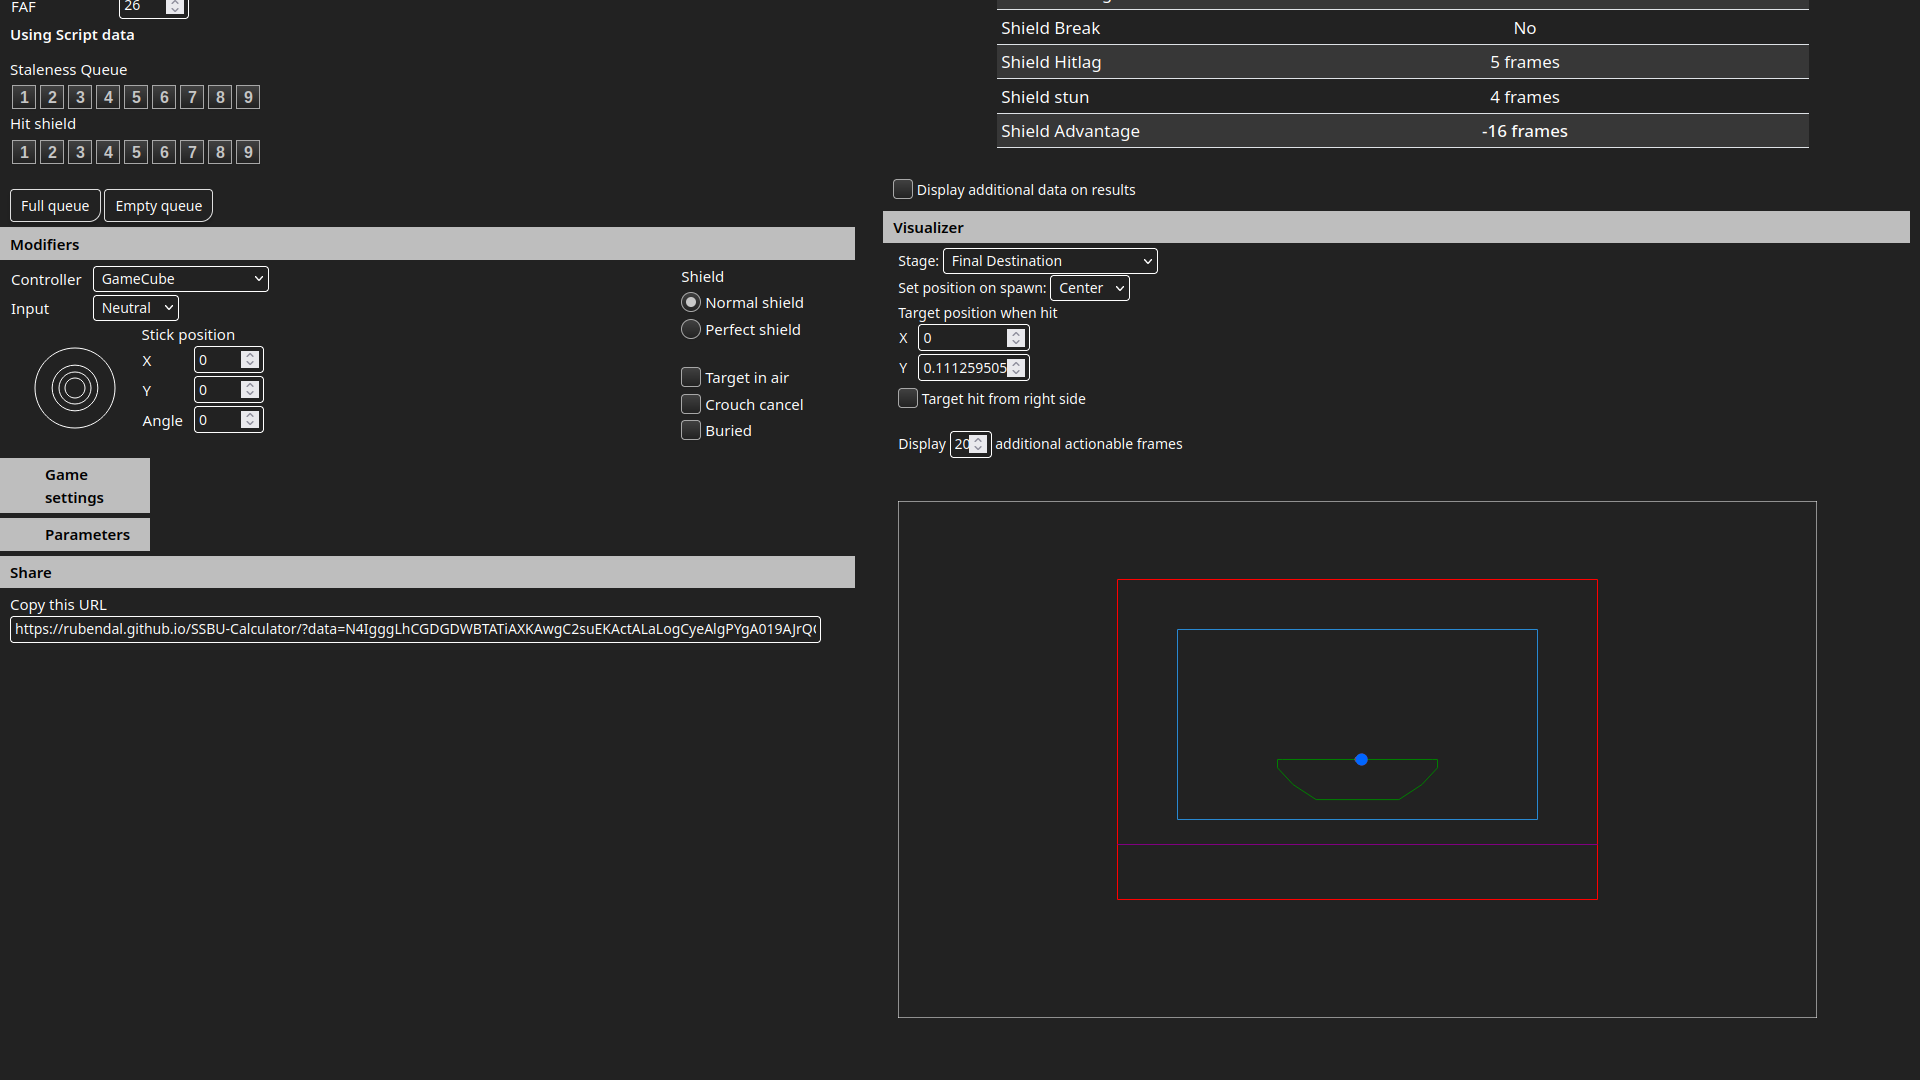
\includegraphics[width=\textwidth]{figures/SUC2.png}
    \caption{Opciones adicionales de \textit{Smash Ultimate Calculator}}
    \label{fig: SUC additional options}
\end{figure}

